\chapter{Task Description and Overview}\label{chapter:task}

\section{Task Description and Overview}
\label{sec:taskdesc}

The first step in our development process was to get a brief overview of
our complete system. To do this, we have followed a conventional style
of designing UML use cases together with a textual description. From
reading this chapter, the reader should be able to understand how our
end product works. The assumptions and constraints that affected our
process are also discussed in section~\ref{sec:assumtions}.
Reading this chapter will be important to
understand the rest of this report.

\section{Assignment}
According to our customer, IDI Open's previous solution was
cumbersome to use. Our assignment was to create a replacement system
that would be easier to administer.
This included replacing both front and back-end systems.

The features of the old solution, in a nutshell, are given below.
\begin{itemize}
\item Website containing information about the contest
\item Team-registration and scoring
\item Ability for users to upload code to be compiled and executed
\end{itemize}

We were given access to the code for the old solution. The customers
felt that this code was cluttered, but we could re-use components
wherever we wanted. However, it was important that we did this in an
structured manner, such that other developers could easily understand the
new solution.

\section{GentleIDI}

Since we were delivering an end product to a real customer, we wanted to
present ourselves as a real company. We chose the name
``GentleCoding'' as our
representative name. This was used to name our repositories, email
lists and other media communicated with external parties.

The term ``Gentle'' is supposed to
represent our calm approach to problems. It is also similar to
``Gentleman'', which reminds of quality and good conduct. Furthermore, it is
easy to interpret and remember.

Since we were developing a new system, we also wanted to brand our product. We
wanted to keep it logical and simple, so we decided on ``GentleIDI''.
Consequently, GentleIDI may be used to refer to our end product throughout the
rest of the report.

\pagebreak
\section{Assumptions and Constraints}
\label{sec:assumtions}
To define what is satisfactory, we have made some assumptions and
defined some constraints. Table~\ref{table:assumtions} should make it easier to
understand how we have reasoned our system design.

\begin{longtable}{|p{.33\textwidth}|p{.33\textwidth}|p{.33\textwidth}|}
\caption[test]{Assumtions and constraints}\label{table:assumtions} \\
\hline \multicolumn{1}{|c|}{\textbf{Assumption/Constraint}} &
\multicolumn{1}{c|}{\textbf{Why}} &
\multicolumn{1}{c|}{\textbf{Implication}} \\
\hline
\endfirsthead

\multicolumn{3}{c}%
{{\bfseries \tablename\ \thetable{} -- continued from previous page}} \\
\hline \multicolumn{1}{|c|}{\textbf{Assumption/Constraint}} &
\multicolumn{1}{c|}{\textbf{Why}} &
\multicolumn{1}{c|}{\textbf{Implication}} \\
\hline
\endhead
The system will be maintained
by people who have experience with computers. & People that are involved with
any programming contest are typically programmers themselves. & User design,
words and definitions can be made more technical. Error messages can be
explained using computer lingo. \\\hline

The system will be used and maintained for {\textgreater} 5 years &
Customer-constraint: they do not want to spend too much time
developing new products, so maintenance is preferred. & The code should be
written in a modular, extensible way with clear documentation.\\\hline

The customer is based at Gløshaugen. & & High availability for customer
meetings and reviews.\\\hline

The developers will maintain a 20 hour a week work ethic throughout the
project{}-duration of 19 weeks. & To finish the product on time.
& The set of requirements should not require more than 20 hours of work per
week per developer, in order to complete.\\\hline
Our system should be user{}-friendly &
Our solution features a web interface available to everyone. Ideally,
any person should be comfortable with the user interface. &
Should have a user{}-friendly interface.
\\\hline
Our end product will be open sourced. &
To ensure quality, and let other volunteers contribute to the code
repository. &
No proprietary third party modules can be used. \ We cannot copyright
our own material. \\\hline
The final product must run on Linux{}-computers. &
This is the choice of OS by NTNU, which is responsible for technical
support and server access. &
Linux{}-compliant solution.\\\hline
We are allowed to use whatever third party plugin we want, as long as it
is free and has no copyright{}-conflict. &
Speed up development. &
Speed up development.\\\hline
\end{longtable}

Do note that the implications in table~\ref{table:assumtions} were not necessarily upheld.
Rather, they were used as initial bounds to permit leeway. For example,
imposing that third party plugins will speed up development does not
mean that we would alway prioritize software re-use.

\section{Roles and Their Definitions}
\subsection{Usergroups}
Within the application-domain of
GentleIDI there are different
groups of users. Each group has different levels of access control, and
once a user is made a member of that group, they inherit those rights.
A user may have membership in all groups. A privileged user is someone
who is given elevated permissions. Table~\ref{table:usegroup} shows the
different roles and their available actions. Further elaborations on
each group will also be given in later sections, but table~\ref{table:usegroup} should
suffice for an overview.

\begin{longtable}{|p{.2\textwidth}|p{.6\textwidth}|}
\caption{Usergroup overview} \label{table:usegroup}\\
\hline
\multicolumn{1}{|c|}{\textbf{ID}} &
\multicolumn{1}{c|}{\textbf{Story}} \\
\hline
Role &
Description\\\hline
Admin &
Privileged. An admin can modify all the available settings of the
system\\\hline
Judge &
Privileged. Similar to an admin account, but with a limited set of
actions: answering questions (clarification system), upload problem to be
solved, solutions to those problems, and incorrect answers (e.g.\ answers
that will provide penalty).\\\hline
Functionary &
Privileged. Functionaries hand out balloons when a team has solved a
problem. To determine what team will be given a balloon, the functionaries
have their own interface with a team overview.\\\hline
Contestants &
A contestant has an account on the system and has the possibility to
enter and compete in a contest. \\\hline
Team &
A group of one to three contestants. A contestant is only part of one
team per contest, and need a team in order to compete. \\\hline

\end{longtable}

\pagebreak
\subsection{Service-providing Units}

Another way of viewing the task description in section~\ref{sec:taskdesc}, is to say
that our solution needs to do three actions: serve web-content, store
data and execute user-submitted code. Since each of these operates with
different protocols, we will think to our solution as composed of three
different systems. These are described in table~\ref{table:serviceUnits}.

\begin{longtable}{|l|m{0.5\textwidth}|m{0.2\textwidth}|}
\caption{Service-providing Units} \label{table:serviceUnits} \\
\hline \multicolumn{1}{|c|}{\textbf{Entity}} &
\multicolumn{1}{c|}{\textbf{Features}} &
\multicolumn{1}{c|}{\textbf{Protocol}} \\
\hline
Webserver & Processes requests from contestants and teams. Also acts as an
interface to the execution node, both receiving and transmitting data
to other execution nodes on the behalf of users. & HTTP\\\hline

Execution node & A service, often on a dedicated platform, that offers the
ability to compile and execute code. The execution node returns output data to
the webserver. & AMQP\\\hline

Database & The storage unit for all user{}-data and logs. & SQL\\\hline
\end{longtable}

\section{UML Use Cases}
We need one page each for privileged, registered, and non-registered
users. That is, one interface for administrative users, one for
contestants, and one for non-registered viewers. From each of these
three, we defined use case scenarios. Figures~\cref{figure:usecasepriv,figure:hei} models the
available workflows and actions for each category of users.
Table~\ref{table:uml-notation} describes the semantics of objects used in the
diagram, which should be equivalent to the UML 2.0 standard.
\begin{longtable}{|m{0.15\textwidth}|m{0.7\textwidth}|}
\caption{UML Notation} \label{table:uml-notation} \\
\hline
	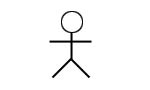
\includegraphics[height=.070\textwidth]{chapter2-img1.jpg}  &
Use case actor. Represents a user group\\\hline
	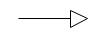
\includegraphics[width=0.15\textwidth]{chapter2-img2.png}  &
UML generalization arrow. Used to indicate inheritance. The
arrow's tail represents the entity that
inherits from where the arrow points to.\\\hline
{\textless}{\textless}include{\textgreater}{\textgreater} &
UML stereotype to represent a mandatory extension to a
workflow.\\\hline
{\textless}{\textless}extend{\textgreater}{\textgreater} &
UML stereotype to indicate that if certain conditions are met in a flow,
the entity to which this arrow points to can extend the
workflow.\\\hline
\end{longtable}

The purpose of the use case diagrams is to give a clear overview of what
users shall be able to accomplish from our system. Furthermore, use
case diagrams are easier to communicate to external parties, such that
it is easier to agree on the system's properties. The
use case diagrams were used early in development to agree on the
requirements specification and to communicate what we
were trying to accomplish.

\begin{figure}[h!]
    \centering
    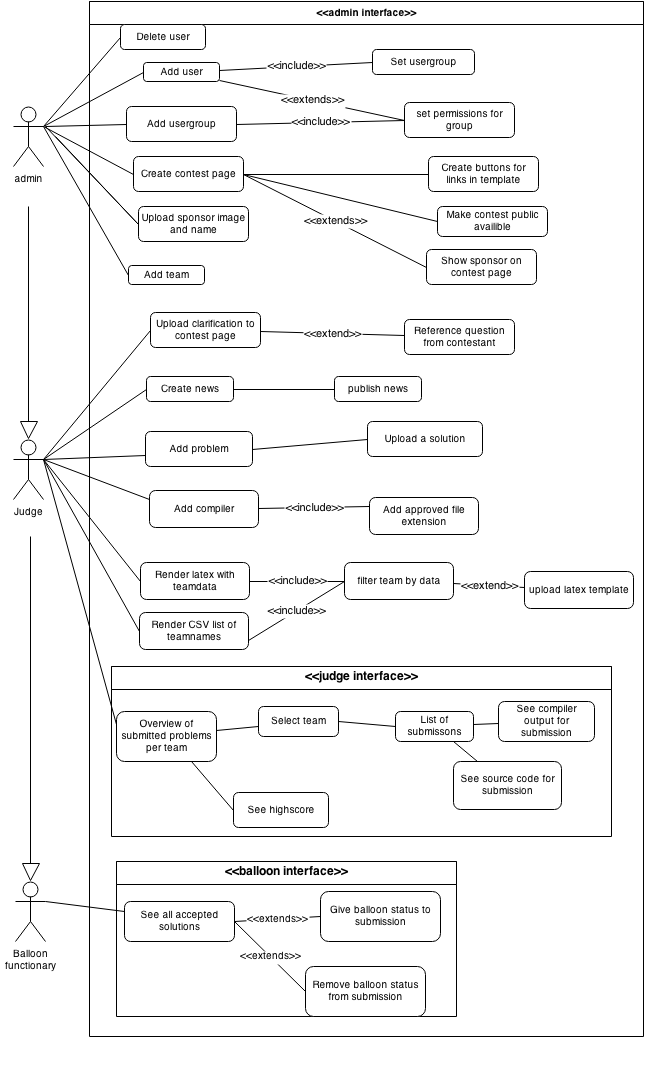
\includegraphics[height=.9\textheight]{UML_use_privileged}
    \caption{UML use case for priviliged users} \label{figure:usecasepriv}
\end{figure}

\begin{figure}[h!]
    \centering
    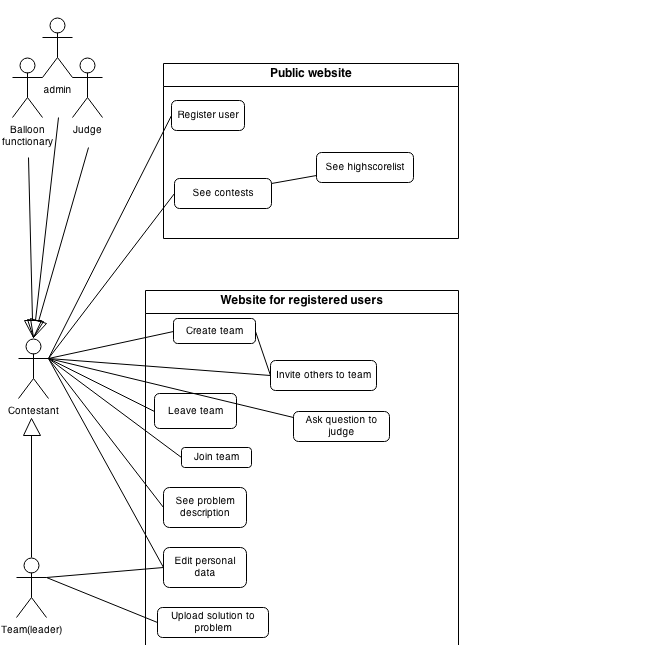
\includegraphics[trim = 0 0 160 0, width=0.6\textwidth]{UML_use_contestant}
    \caption{UML use case for non-privileged users} \label{figure:hei}
\end{figure}
As seen in figures~\cref{figure:usecasepriv,figure:hei}, admins
has privileges to perform the actions of any other group, in addition to
their own set of actions. Thus, membership in the admin group gives a user
complete control in the application domain. Furtherly, it can be noted that
all usergroups have the opportunity to act as a contestant to review the
website. Privileged users will are still restricted from appearing in the
official high score tables to prevent them from assuming a competing role.
This was to avoid the chance of any person with access to the solutions to
compete.
